\usetikzlibrary{calc}

\begin{frame}{OSI model}
\begin{tikzpicture}
\node (osi) at (0,0) {
    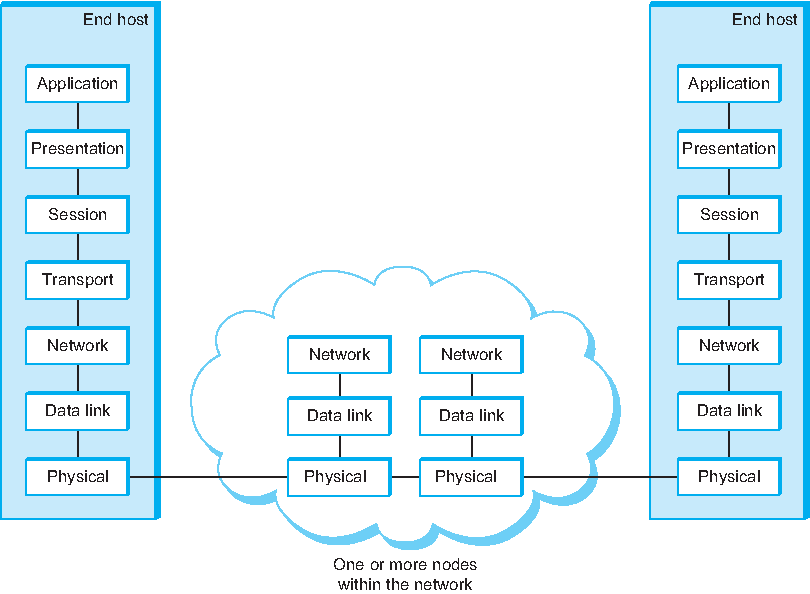
\includegraphics[height=0.75\textheight]{../intro/systemsapproach-1-fig-13.pdf}
};
\coordinate[overlay] (explain loc) at ([yshift=1cm,xshift=0cm]osi.north east);
\tikzset{
    explain box/.style={font=\small,alt=<2>{draw=red}{draw=black},very thick,align=left,at={(explain loc)}, anchor=north west},
    alt explain box/.style={draw=red,ultra thick,anchor=north east,align=left,at={([yshift=-1cm]explain loc)},fill=white},
}
\begin{visibleenv}<2->
\node[overlay,explain box] {
    (7) \myemph<3>{application}: \\ \hspace{.5cm}what requests/etc. \\
    (6) \myemph<3>{presentation}: \\ \hspace{.5cm}data format \\
    (5) \myemph<3>{session}: \\ \hspace{.5cm}manage group of streams \\
    (4) transport: \\ \hspace{.5cm}streams of data \\
    (3) network: \\ \hspace{.5cm}message to correct network \\
    (2) data link: \\ \hspace{.5cm}message $\rightarrow$ bits \\
    \hspace{.5cm}message to correct machine \\
    (1) physical: \\ \hspace{.5cm}send bits/\ldots 
};
\end{visibleenv}
\begin{visibleenv}<3>
\node[overlay,alt explain box] {
    current Internet \\
    usually* layers 5--7 merged together
};
\end{visibleenv}
\end{tikzpicture}
\imagecredit{Figure 13 of Chapter 1 of Computer Networks: A Systems Approach (6th ed) (Peterson and Davie)}
\end{frame}

\begin{frame}<0>{OSI model (text)}
\begin{tabular}{lll} \hline
7 & \myemph<2>{application} & what requests/etc. \\ \hline 
6 & \myemph<2>{presentation} & format of data \\ \hline 
5 & \myemph<2>{session} & coordinate multiple streams \\ \hline
4 & transport & streams of data \\ \hline
3 & network & message to correct network \\ \hline
2 & data link & message to correct machine \\ 
~ & ~ & message into bits/symbols \\
1 & physical & transmit bits/symbols on medium \\
\end{tabular}
\begin{itemize}
\item<2-> \myemph<2>{internet: usually combines layers 7/6/5}
\end{itemize}
\end{frame}

\begin{frame}{OSI model}
    \begin{itemize}
    \item standardized by ISO (International Standards Organization) and ITU (International Telecommunications Union)
    \item full set of protocols\ldots
        \begin{itemize}
        \item file transfer, message sending, directory lookups \ldots
        \end{itemize}
    \item that were often implemented and sometimes used\ldots
    \item but mostly lost out to IETF-standardized Internet protocols
        \begin{itemize}
        \item Internet Engineering Task Force
        \end{itemize}
    \end{itemize}
\end{frame}

\begin{frame}{OSI influence (1)}
    \begin{itemize}
    \item term `layer 7', `layer 4', `layer 3', etc. almost always refer to OSI model
    \item \ldots even though most of Internet does not follow it
        \begin{itemize}
        \item early Internet protocols predate OSI
        \end{itemize}
    \end{itemize}
\end{frame}

\begin{frame}{OSI influence (2)}
    \begin{itemize}
    \item are a lot of Internet protocols influenced by OSI protocols
    \vspace{.5cm}
    \item OSI's DAP (directory access protocol) 
        \begin{itemize}
        \item adapted into IETF's LDAP (lightweight directory access protocol)
        \end{itemize}
    \item OSI presentation layer ASN.1 used in\ldots
        \begin{itemize}
        \item telephony (between telephone companies)
        \item inter-bank messaging
        \item lots of cryptography-related protocols
        \item \ldots
        \end{itemize}
    \item OSI's routing protocol IS-IS still common in large Internet-connected networks
        \begin{itemize}
        \item (adapted to work alongside IETF protocols)
        \end{itemize}
    \end{itemize}
\end{frame}

\begin{frame}{Internet layers}
\small
\begin{tabular}{|l|l|l|p{6cm}|} 
OSI layer & name & examples & purpose \\ \hline
7 & application & HTTP, SSH, & {application-defined meanings}\\
~ & ~ & SMTP, DNS, \ldots & ~ \\ \hline
4 & {transport} & TCP, UDP, \ldots & {reach correct program,\linebreak \myemph<2>{reliablity/streams}} \\ \hline
3 & {network} & IPv4, IPv6, \ldots & {reach correct machine}\linebreak(across networks) \\ \hline
2 & {link} & Ethernet, Wi-Fi, \ldots & {coordinate shared wire/radio}\\ \hline
1 & physical & \ldots & encode bits for wire/radio \\ \hline
\end{tabular}
\end{frame}

\begin{frame}{Internet protocols and layers (non-exhaustive)}
\begin{tikzpicture}
\node[anchor=north west] (int) at (0,0) {
    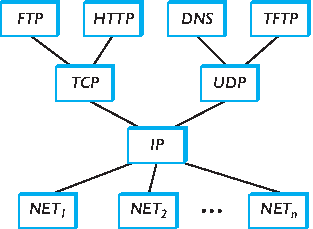
\includegraphics[height=0.75\textheight]{../intro/systemsapproach-1-fig-14.pdf}
};
%\draw[help lines] (0, 0) grid (14, -8);
%\draw[step=2,draw,thick,red] (0, 0) grid (14, -8);
\tikzset{
    layer hi/.style={draw=red,ultra thick},
    layer label/.style={anchor=west},
}
\draw[layer hi] (0, 0) rectangle (9, -1.3);
\node[layer label] at (9.1, -0.65) { application {\it\small OSI layer 7} };
\draw[layer hi] (1.5, -1.8) rectangle (7.5, -3.2);
\node[layer label] at (8.6, -2.5) { transport {\it\small OSI layer 4} };
\draw[layer hi,alt=<2>{fill=red,fill opacity=0.1}] (3.5, -3.6) rectangle (5.6, -4.85);
\node[layer label] at (5.8, -4.2) (net label) { network {\it\small OSI layer 3} };
\draw[layer hi] (0.5, -5.5) rectangle (9, -6.6);
\node[layer label] at (9.1, -6) { data link {\it\small OSI layer 2} };
\begin{visibleenv}<2>
    \node[anchor=west,red,font=\large] at (net label.east) {``narrow waist''};
\end{visibleenv}
\end{tikzpicture}
\imagecredit{Figure 14 of Chapter 1 of Computer Networks: A Systems Approach (6th ed) (Peterson and Davie)}
\end{frame}

